\documentclass[11pt]{article}
% ===== Préambule commun aux documents Séries Chronologiques =====
\usepackage[utf8]{inputenc}
\usepackage[T1]{fontenc}
\usepackage[french]{babel}
\usepackage{lmodern}
\usepackage{amsmath,amssymb,amsthm,mathtools}
\usepackage{geometry}
\geometry{a4paper,margin=2.3cm}
\usepackage{enumitem}
\usepackage{array,booktabs,longtable}
\usepackage{xcolor}
\usepackage[most]{tcolorbox}
\usepackage{etoolbox}
\usepackage{graphicx}
\graphicspath{{figs/}}
\usepackage{caption}
\captionsetup{font=small,labelfont={bf,color=insea}}
\usepackage{fancyhdr}
\usepackage{titlesec}
\usepackage{hyperref}
\hypersetup{colorlinks=true,linkcolor=blue!55!black,urlcolor=blue!55!black,
  citecolor=blue!55!black,bookmarksopen=true}
\usepackage{bookmark}

% --- Couleurs ---
\definecolor{insea}{RGB}{0,76,128}
\definecolor{insealight}{RGB}{232,240,247}
\definecolor{vert}{RGB}{0,120,70}
\definecolor{vertlight}{RGB}{232,245,238}
\definecolor{orange}{RGB}{190,90,0}
\definecolor{orangelight}{RGB}{252,242,228}
\definecolor{gris}{RGB}{90,90,90}

% --- En-têtes / pieds ---
\pagestyle{fancy}
\fancyhf{}
\fancyhead[L]{\small\color{gris}\leftmark}
\fancyhead[R]{\small\color{gris}Séries Chronologiques}
\fancyfoot[C]{\thepage}
\renewcommand{\headrulewidth}{0.4pt}
\renewcommand{\footrulewidth}{0pt}

% --- Titres de section colorés ---
\titleformat{\section}{\Large\bfseries\color{insea}}{\thesection.}{0.6em}{}
\titleformat{\subsection}{\large\bfseries\color{insea!85!black}}{\thesubsection.}{0.6em}{}
\titleformat{\subsubsection}{\bfseries\color{gris}}{\thesubsubsection.}{0.6em}{}

% --- Théorèmes (pour le cours) ---
\theoremstyle{definition}
\newtheorem{definition}{Définition}[section]
\newtheorem{exemple}{Exemple}[section]
\newtheorem{remarque}{Remarque}[section]
\newtheorem{methode}{Méthode}[section]
\theoremstyle{plain}
\newtheorem{theoreme}{Théorème}[section]
\newtheorem{proposition}{Proposition}[section]
\newtheorem{corollaire}{Corollaire}[section]
\newtheorem{propriete}{Propriété}[section]

% --- Boîtes ---
\newtcolorbox{recette}[1][]{colback=vertlight,colframe=vert,
  fonttitle=\bfseries,title={Recette d'examen\ifblank{#1}{}{ --- #1}}}
\newtcolorbox{attention}[1][]{colback=orangelight,colframe=orange,
  fonttitle=\bfseries,title={Attention\ifblank{#1}{}{ --- #1}}}
\newtcolorbox{rappel}[1][]{colback=insealight,colframe=insea,
  fonttitle=\bfseries,title={Rappel de cours\ifblank{#1}{}{ --- #1}}}
\newtcolorbox{reponse}[1][]{colback=vertlight,colframe=vert!70!black,
  left=2mm,right=2mm,top=1mm,bottom=1mm,boxrule=0.8pt,#1}

% --- Notations Séries Chronologiques ---
\newcommand{\E}{\mathbb{E}}
\newcommand{\Var}{\operatorname{Var}}
\newcommand{\Cov}{\operatorname{Cov}}
\newcommand{\Corr}{\operatorname{Corr}}
\newcommand{\cor}{\operatorname{cor}}
\newcommand{\BB}{\operatorname{BB}}
\newcommand{\R}{\mathbb{R}}
\newcommand{\Z}{\mathbb{Z}}
\newcommand{\N}{\mathbb{N}}
\newcommand{\Xhat}{\widehat{X}}
\newcommand{\phihat}{\widehat{\phi}}
\newcommand{\rhohat}{\widehat{\rho}}
\newcommand{\gammahat}{\widehat{\gamma}}
\newcommand{\eps}{\varepsilon}
\DeclareMathOperator{\sgn}{sgn}

% Étiquette « bonne réponse » pour les QCM (utilisée dans le corrigé)
\newcommand{\bonne}[1]{\textbf{\color{vert}#1}}
\newcommand{\horsprog}{\textsuperscript{\color{orange}\,$\star$}}


\title{\vspace{-1cm}\textbf{\color{insea}Séries Chronologiques}\\[2mm]
\large Recueil de questions et d'exercices d'examens\\[1mm]
\normalsize (énoncés \emph{contextualisés et corrigés}, classés par thème, sans doublons)}
\author{Préparation au module --- d'après le cours de F.~BADAOUI (INSEA)}
\date{\today}

\newtcolorbox{contexte}[1][]{colback=insealight,colframe=insea!70!black,
  left=2mm,right=2mm,top=1mm,bottom=1mm,boxrule=0.6pt,
  fonttitle=\bfseries\small,title={Contexte\ifblank{#1}{}{ --- #1}}}

\begin{document}
\maketitle
\thispagestyle{empty}

\begin{tcolorbox}[colback=insealight,colframe=insea,title={À propos de ce document}]
Ce recueil rassemble \textbf{toutes} les questions de \texttt{sc.txt}. Chaque énoncé a été
\textbf{reformulé pour être autonome} (rappel du cadre, données complètes, notations
explicites), \textbf{corrigé} de ses coquilles d'OCR, puis \textbf{classé par thème} et
\textbf{dédoublonné}. Les corrigés \emph{très détaillés} sont dans \emph{Solutions\_SC.pdf}
(même numérotation). Les questions \horsprog{} hors-programme sont en dernière section.

\smallskip\noindent\textbf{Conventions.} $B$ : opérateur retard ($B^kX_t=X_{t-k}$) ;
$a_t$ (ou $\eps_t$) : bruit blanc $\BB(0,\sigma^2)$ ; un modèle ARMA s'écrit
$\Phi(B)X_t=\mu+\Theta(B)a_t$ avec $\Phi(B)=1-\phi_1B-\dots$, $\Theta(B)=1-\theta_1B-\dots$
\end{tcolorbox}

\tableofcontents
\newpage

% =====================================================================
\section{QCM théoriques et questions de cours}
\markboth{QCM théoriques}{}
\begin{contexte}
Ces questions portent sur les \emph{définitions} et \emph{propriétés qualitatives} du cours
(décomposition, filtres, caractérisation ACF/PACF des modèles, validation). Sauf mention
contraire, une seule réponse est correcte.
\end{contexte}

\subsection{Concepts de base et décomposition}
\begin{enumerate}[label=\textbf{Q\,A.\arabic*},leftmargin=*]
\item Un processus \textbf{stationnaire} (au sens large) sert à modéliser :
\begin{enumerate}[label=\Alph*.,nosep]
  \item des séries qui \emph{ne peuvent pas} présenter de tendance ni de saisonnalité ;
  \item des séries présentant une tendance ;
  \item des séries présentant une saisonnalité ;
  \item des séries présentant une tendance \emph{et} une saisonnalité.
\end{enumerate}

\item Une \textbf{moyenne mobile} est :
\begin{enumerate}[label=\Alph*.,nosep]
  \item un filtre non linéaire ; \quad B. un filtre linéaire, pas forcément centré ni symétrique ;
  \item un filtre linéaire centré, pas forcément symétrique ; \quad D. un filtre linéaire normalisé.
\end{enumerate}

\item La \textbf{moyenne mobile MM4} (centrée), appliquée à une série trimestrielle :
\begin{enumerate}[label=\Alph*.,nosep]
  \item absorbe les tendances linéaires et conserve les saisonnalités de période 4 ;
  \item absorbe les tendances linéaires et conserve les saisonnalités de période paire ;
  \item conserve les tendances linéaires et absorbe les saisonnalités de période 4 ;
  \item conserve les tendances linéaires et absorbe les saisonnalités de période impaire.
\end{enumerate}

\item L'algorithme \textbf{X11} de désaisonnalisation \emph{(plusieurs réponses possibles)} :
\begin{enumerate}[label=\Alph*.,nosep]
  \item contient des boucles itératives pour évaluer la série CVS ;
  \item est l'algorithme le plus sophistiqué connu à l'heure actuelle ;
  \item combine régression linéaire et moyennes mobiles.
\end{enumerate}

\item \textbf{Vrai / Faux.} La décomposition d'une série chronologique sert \emph{essentiellement}
à retrancher à la série sa seule saisonnalité.

\item \textbf{Vrai / Faux.} La première moyenne mobile utilisée pour extraire les variations
saisonnières doit conserver la tendance et réduire la variance du bruit.

\item \textbf{Vrai / Faux.} La prévision par \emph{lissage exponentiel simple} ne tient pas
compte de la saisonnalité.

\item La méthode de \textbf{Holt--Winters} \emph{(plusieurs réponses possibles)} :
\begin{enumerate}[label=\Alph*.,nosep]
  \item est plus complète que les lissages exponentiels simple ou double ;
  \item tient compte d'une saisonnalité mais pas d'une tendance ;
  \item tient compte d'une tendance \emph{et} d'une saisonnalité.
\end{enumerate}
\end{enumerate}

\subsection{Caractérisation des processus AR, MA, ARMA, SARIMA}
\begin{enumerate}[label=\textbf{Q\,A.\arabic*},leftmargin=*,start=9]
\item Un processus \textbf{AR} est caractérisé par :
\begin{enumerate}[label=\Alph*.,nosep]
  \item ACF et PACF s'annulant à partir d'un certain rang ;
  \item ACF décroissant vers 0 et PACF s'annulant à partir d'un certain rang ;
  \item ACF s'annulant à partir d'un certain rang et PACF décroissant vers 0.
\end{enumerate}
\item Un processus \textbf{ARMA} (avec $p\ge1$ et $q\ge1$) est caractérisé par :
\begin{enumerate}[label=\Alph*.,nosep]
  \item ACF et PACF s'annulant à partir d'un certain rang ;
  \item ACF s'annulant à partir d'un certain rang ; \quad C. PACF s'annulant à partir d'un certain rang ;
  \item aucune des propriétés précédentes (les deux décroissent sans s'annuler).
\end{enumerate}
\item Un processus \textbf{SARIMA} :
\begin{enumerate}[label=\Alph*.,nosep]
  \item est stationnaire ; \quad B. modélise une tendance mais pas de saisonnalité ;
  \item modélise une saisonnalité mais pas de tendance ;
  \item modélise une tendance \emph{et/ou} une saisonnalité.
\end{enumerate}
\item \textbf{Vrai / Faux.} Tout processus MA stationnaire possède une représentation AR.
\item Pour \textbf{valider un modèle ARMA}, on vérifie \emph{(plusieurs réponses possibles)} :
\begin{enumerate}[label=\Alph*.,nosep]
  \item la significativité des paramètres ; \quad B. la blancheur des résidus ;
  \item la normalité des résidus.
\end{enumerate}
\item \textbf{Vrai / Faux.} Si $X_t$ est stationnaire, la statistique de Ljung--Box calculée
sur $X_t$ (et non sur les résidus d'un modèle) devrait nous conduire à accepter l'hypothèse
nulle qui lui est associée.
\end{enumerate}

\subsection{Questions de cours (à développer)}
\begin{enumerate}[label=\textbf{Q\,A.\arabic*},leftmargin=*,start=15]
\item Citer deux types de stationnarité. Laquelle est la plus pratique, et pourquoi ?
\item À quelle condition un processus strictement stationnaire est-il stationnaire au second
ordre ?
\item Que permet d'identifier un corrélogramme (ACF empirique) ?
\item Caractériser un AR$(p)$ par sa fonction d'autocorrélation partielle.
\item Citer et expliquer deux tests de validation d'un modèle ARMA gaussien.
\item Donner un critère de qualité \emph{prédictive} d'un modèle ARMA.
\item Citer et expliquer deux critères de \emph{sélection} d'un AR$(p)$ gaussien.
\end{enumerate}

% =====================================================================
\section{Stationnarité, causalité et inversibilité}
\markboth{Stationnarité, causalité, inversibilité}{}
\begin{contexte}
On rappelle : un AR est \emph{stationnaire (causal)} ssi les racines de $\Phi(B)=0$ sont de
module $>1$ ; un MA est \emph{inversible} ssi les racines de $\Theta(B)=0$ le sont.
Bien penser à \emph{simplifier les racines communes} avant de conclure.
\end{contexte}
\begin{enumerate}[label=\textbf{Q\,B.\arabic*},leftmargin=*]
\item Soit $z$ une variable aléatoire d'espérance nulle et de variance unité, et la série
$X_t=(-1)^t z$. Calculer $\E(X_t)$ et $\gamma(k)=\Cov(X_t,X_{t+k})$, puis dire si $(X_t)$ est
stationnaire au sens large.

\item Soit $X_t=0.8X_{t-1}-0.15X_{t-2}+a_t-0.3a_{t-1}$, $a_t$ bruit blanc. Le processus
est-il \emph{(a)} stationnaire et inversible ; \emph{(b)} stationnaire et non inversible ;
\emph{(c)} non stationnaire et inversible ; \emph{(d)} non stationnaire et non inversible ?
Justifier en étudiant les racines.

\item \textbf{Vrai / Faux} (justifier). Le processus $(1-1.66B+0.66B^2)X_t=(1-B)a_t$
possède une représentation AR \emph{d'ordre fini}. \emph{(Indication : factoriser les deux
polynômes.)}

\item \textbf{Vrai / Faux} (justifier). Le processus $X_t=1.6X_{t-1}-0.6X_{t-2}+a_t-0.6a_{t-1}$
est stationnaire.

\item Soit $(1-0.8B)X_t=(1+0.4B)a_t$ (ARMA(1,1)).
\begin{enumerate}[label=\alph*.,nosep]
  \item Possède-t-il une représentation AR ? (non / ordre fini / ordre infini). Justifier.
  \item Possède-t-il une représentation MA ? (non / ordre fini / ordre infini). Justifier.
\end{enumerate}

\item Le processus $X_t=0.8X_{t-1}+a_t+0.8a_{t-1}$ est-il stationnaire ? inversible ?

\item Pour chacun des processus suivants ($(\eps_t)$ bruit blanc de variance $\sigma^2>0$),
dire en justifiant s'il est \emph{centré} et/ou \emph{stationnaire} et/ou \emph{de type ARIMA}
(préciser les ordres) :
\[
\text{1) }X_t=\eps_t-\eps_{t-3};\quad \text{2) }X_t+\eps_t^2=\sigma^2;\quad
\text{3) }X_t-X_{t-2}=\eps_t;\quad \text{4) }X_t=2t+\eps_t-\eps_{t-2}.
\]

\item Soit $X_t-aX_{t-1}=\eps_t$, $0<|a|<1$, $(\eps_t)$ bruit blanc de variance $\sigma^2$.
\emph{1)} Reconnaître le processus ; est-il causal ? \emph{2)} Exprimer $X_t$ en fonction des
$(\eps_t)$. \emph{3)} Si les $\eps_t$ sont i.i.d.\ gaussiens, que dire de $(X_t)$ ?

\item Soit $X_t-aX_{t-1}=\eps_t-2b\eps_{t-1}+b^2\eps_{t-2}$, $(\eps_t)$ bruit blanc.
\emph{i)} Reconnaître le processus ; est-il causal ? \emph{ii)} Quand est-il inversible ?
Exprimer alors $\eps_t$ en fonction des $(X_t)$. \emph{(Indication : $\Theta(B)=(1-bB)^2$.)}

\item \emph{(Examen 22/12/2011.)} Soit $X_t$ stationnaire de moyenne nulle, $\alpha,\beta\in\R$
et $s_t$ une saisonnalité de période 12. Montrer que :
\emph{1)} si $Z_t=\alpha+\beta t+s_t+X_t$ alors $(1-B)(1-B^{12})Z_t$ est stationnaire ;
\emph{2)} si $Z_t=(\alpha+\beta t)s_t+X_t$ alors $(1-B^{12})^2Z_t$ est stationnaire.

\item \emph{(Examen 22/12/2011.)} Soit l'AR(1) $X_t=\alpha X_{t-1}+a_t$, $|\alpha|<1$, et
$Y_t=X_{2t}$ (sous-échantillonnage). Montrer que $Y_t=\phi Y_{t-1}+b_t$ avec $b_t$ bruit
blanc et $\phi$ à identifier ; conclure que $(Y_t)$ est un AR(1) stationnaire causal.

\item Soit $(1-\phi B^2)Y_t=\delta+(1+\theta B)a_t$.
\emph{1)} Déterminer la suite $(\psi_j)$ de la forme $Y_t=\sum_{j\ge0}\psi_j a_{t-j}$.
\emph{2)} Conditions sur $\phi,\theta$ pour la stationnarité et la causalité.
\emph{3)} Calculer $\rho(1)$.
\end{enumerate}

% =====================================================================
\section{Représentations \texorpdfstring{$\mathrm{MA}(\infty)$ et $\mathrm{AR}(\infty)$}{MA-inf et AR-inf}}
\markboth{Représentations MA-infini et AR-infini}{}
\begin{contexte}
On cherche les coefficients $\psi_k$ (forme $X_t=\sum_k\psi_k a_{t-k}$, MA$\infty$) ou
$\pi_k$ (forme $a_t=\sum_k\pi_k X_{t-k}$, AR$\infty$). \textbf{Méthode} : identifier les
coefficients de $B^k$ dans $\Phi(B)\Psi(B)=\Theta(B)$ (pour $\psi$) ou
$\Theta(B)\Pi(B)=\Phi(B)$ (pour $\pi$).
\end{contexte}
\begin{enumerate}[label=\textbf{Q\,C.\arabic*},leftmargin=*]
\item Soit l'AR(2) $X_t-0.9X_{t-1}+0.2X_{t-2}=a_t$. Déterminer $\psi_1,\psi_2,\psi_3$ puis la
forme générale de $\psi_k$ ($k\ge0$) de la représentation $X_t=\sum_{k\ge0}\psi_k a_{t-k}$.

\item Soit $X_t=0.6X_{t-1}+0.2X_{t-2}+a_t-0.5a_{t-1}$. Donner les \emph{quatre} premiers
coefficients $\pi_0,\pi_1,\pi_2,\pi_3$ de la représentation autorégressive
($\mathrm{AR}(\infty)$).

\item Soit $(1-0.8B)X_t=(1+0.4B)a_t$. Donner \emph{(a)} les trois premiers coefficients de la
représentation $\mathrm{AR}(\infty)$ ; \emph{(b)} les trois premiers coefficients de la
représentation $\mathrm{MA}(\infty)$.

\item Sur données journalières, $(1-\Phi_1 B^7)x_t=a_t$ ($a_t$ bruit blanc de variance
$\sigma^2$, $|\Phi_1|<1$). \emph{a)} Écriture $\mathrm{MA}(\infty)$. \emph{b)}
$\gamma_0=\Var(x_t)$ en fonction de $\Phi_1,\sigma^2$. \emph{c)} Autocorrélations
$\rho_1,\rho_7,\rho_8,\rho_{14}$. \emph{d)} Autocorrélations partielles
$P_1,P_7,P_8,P_{14}$.

\item Soit l'AR(2) $X_t-0.9X_{t-1}+0.2X_{t-2}=a_t$. \emph{1)} Stationnaire ? \emph{2)}
Calculer $\rho_1,\rho_2$. \emph{3)} En déduire $\rho_k$ pour $k\ge3$. \emph{4)} Déterminer
$\psi_k$ ($\mathrm{MA}(\infty)$).

\item \emph{(Rattrapage 2024--2025, corrigé.)} Soit l'ARMA(1,1)
$x_t=\phi x_{t-1}+a_t-\theta a_{t-1}$, $|\phi|<1$, $a_t$ bruit blanc gaussien. On a relevé le
début de sa représentation $\mathrm{MA}(\infty)$, $x_t=\sum_{k\ge0}\psi_k a_{t-k}$ :
\[
\psi_0=1,\quad \psi_1=0.3,\quad \psi_2=0.15,\quad \psi_3=0.075,\quad \psi_4=0.0375,\ \dots
\]
Déterminer $\phi$ et $\theta$.
\end{enumerate}

% =====================================================================
\section{Autocorrélations simples (ACF) et partielles (PACF)}
\markboth{Autocorrélations ACF / PACF}{}
\begin{contexte}
Outils : pour un AR$(p)$, équations de Yule--Walker $\rho(k)=\sum_j\phi_j\rho(k-j)$ et la PACF
qui \emph{coupe} à $p$ ($P_p=\phi_p$) ; pour un MA$(q)$, l'ACF qui \emph{coupe} à $q$.
\end{contexte}
\begin{enumerate}[label=\textbf{Q\,D.\arabic*},leftmargin=*]
\item $X_t$ est un AR(2) causal solution de $X_t-\phi_1X_{t-1}+\phi_2X_{t-2}=a_t$.
On observe $\rho(1)=0.84$, $\rho(2)=0.69$, $\rho(3)=0.52$, et l'estimation a donné le polynôme
$(1-0.85B+0.32B^2)$ (donc $\phi_1=0.85$, $\phi_2=-0.32$).
\emph{1)} Quelles valeurs des deux premières autocorrélations \emph{partielles}
$\phi_{11},\phi_{22}$ doit-on avoir ? \emph{2)} Exprimer $\rho(1),\rho(2)$ en fonction de
$\phi_1,\phi_2$. \emph{3)} Calculer $\rho(1),\rho(2)$.

\item Soit $(1-0.8B^2)X_t=a_t$. Calculer $\rho_1,\rho_2$ et les autocorrélations partielles
$P_1,P_2$.

\item Calculer les trois premières autocorrélations simples $\rho_1,\rho_2,\rho_3$ du
processus $X_t=0.6X_{t-1}+0.8X_{t-2}-0.3X_{t-3}+a_t$, $a_t\sim\BB(0,1)$. \emph{(On vérifiera
d'abord la stationnarité.)}

\item Soit l'AR(2) $X_t-0.9X_{t-1}+0.2X_{t-2}=a_t$. Calculer $\rho_1,\rho_2$, puis $\rho_k$
pour $k\ge3$.

\item Sur 100 observations, on a obtenu les corrélogrammes (ACF $\rho_k$ et PACF $P_k$) :
\begin{center}\small
\begin{tabular}{cccccc}\toprule
$k$&1&2&3&4&5\\\midrule
$\rho_k$&0.65&0.47&0.35&0.24&0.18\\
$P_k$&0.65&$-0.31$&$-0.08$&$-0.15$&0.10\\\bottomrule
\end{tabular}
\end{center}
Quel modèle ARMA$(p,q)$ retenez-vous ? Justifier (bande $\pm2/\sqrt{100}=\pm0.2$).

\item Une entreprise vend deux produits indépendants : les ventes $x_t$ du premier suivent un
AR(1), celles $y_t$ du second un MA(1). De quel type ARMA$(p,q)$ sont les recettes totales
$z_t=x_t+y_t$ ?
\end{enumerate}

% =====================================================================
\section{Prévision et intervalles de confiance}
\markboth{Prévision et intervalles de confiance}{}
\begin{contexte}
\textbf{Règle} : $\widehat X_{n+h}=\E[X_{n+h}\mid$ passé$]$ : chocs futurs $\to0$, chocs
passés $\to$ résidus, $X$ futurs $\to$ prévisions. Erreur :
$\Var(\Delta_h)=\sigma^2\sum_{j=0}^{h-1}\psi_j^2$ ; IC 95\% :
$\widehat X_{n+h}\pm1.96\,\sigma\sqrt{\sum_{j<h}\psi_j^2}$.
\end{contexte}
\begin{enumerate}[label=\textbf{Q\,E.\arabic*},leftmargin=*]
\item MA(1) $X_t=2+a_t+0.8a_{t-1}$, $a_t$ bruit blanc gaussien de variance $2$ ; on connaît
$a_t=1.6$, $a_{t-1}=-3.4$. \emph{a)} Prévisions pour $t+1$ et $t+2$. \emph{b)} IC à 95\%.

\item Soit $(1-0.8B)X_t=2+a_t$ (i.e.\ $X_t=2+0.8X_{t-1}+a_t$), $a_t$ bruit blanc gaussien de
variance $1$. On connaît $a_T=1.6$ et $X_{T-1}=3.0$. \emph{a)} Prévisions $\widehat X_{T+1}$,
$\widehat X_{T+2}$. \emph{b)} IC à 95\%.

\item MA(2) $Y_t=a_t+0.8a_{t-1}+0.4a_{t-2}$, $a_t\sim N(0,1)$. Dernières observations
$Y_{100}=2.5,Y_{99}=1.8,Y_{98}=0.9$ ; résidus $\hat a_{100}=0.6,\hat a_{99}=-0.3,\hat
a_{98}=0.1$. \emph{a)} Calculer $\widehat Y_{101},\widehat Y_{102},\widehat Y_{103}$.
\emph{b)} Variances d'erreur et IC à 95\%.

\item On donne une série $X_t$ et un modèle MA(1) ajusté par EViews (où la constante
$C$ est la \emph{moyenne} et le modèle s'écrit $X_t=C+a_t+\theta\,a_{t-1}$, $a_t\sim N(0,1)$) :
\begin{center}\small
\begin{tabular}{lcccc}\toprule
$t$ & 06/2012 & 07/2012 & 08/2012 & 09/2012\\ $x_t$ & 1.2 & 3.5 & 4.2 & 6.4\\\bottomrule
\end{tabular}\qquad
\begin{tabular}{lc}\toprule
$C$ & $1.996780$\\ MA(1) ($\theta$) & $-0.492396$\\\bottomrule
\end{tabular}
\end{center}
Calculer la meilleure prévision, la variance d'erreur et l'IC à 95\% pour $X_{10/2012}$,
$X_{11/2012}$, $X_{12/2012}$.

\item \emph{(Série 2, Ex.~1.)} Modèle ARMA(1,1) \emph{sans constante}
$X_t=\phi X_{t-1}+a_t+\theta a_{t-1}$, $\hat\phi=0.495639$, $\hat\theta=0.413047$, sur :
\begin{center}\small
\begin{tabular}{lccccc}\toprule
$t$&2007&2008&2009&2010&2011\\ $X_t$&1.5&1.9&3.2&2.2&2.4\\\bottomrule
\end{tabular}
\end{center}
Calculer $\widehat X_{2012}$ et $\widehat X_{2013}$ (on prendra $a_{2007}=0$ pour amorcer les
résidus).

\item \emph{(Série 2, Ex.~2.)} Modèle AR(1) à moyenne, $C=\mu=7.124608$, $\hat\phi=0.297718$,
$a_t\sim N(0,1)$, sur :
\begin{center}\small
\begin{tabular}{lcccc}\toprule
$t$&2008&2009&2010&2011\\ $x_t$&11.2&13.5&11.2&10.4\\\bottomrule
\end{tabular}
\end{center}
Calculer la meilleure prévision, la variance d'erreur et l'IC à 95\% pour
$X_{2012},X_{2013},X_{2014}$.

\item \emph{(Brouillon reconstitué.)} À partir des observations $X_{2008}=13.5$,
$X_{2009}=11.2$, $X_{2010}=10.9$, $X_{2011}=7.12$ et d'un AR(1) d'intercept $5.0552$ et de
coefficient $0.29$ ($\sigma^2=1$), prévoir $X_{2012},X_{2013},X_{2014}$ avec IC à 95\%.
\end{enumerate}

% =====================================================================
\section{Intégration, ARIMA et tests de Dickey--Fuller}
\markboth{Intégration, ARIMA, Dickey--Fuller}{}
\begin{contexte}
Un processus est intégré d'ordre $d$ si $\Phi(B)$ admet la racine $B=1$ avec multiplicité $d$
(test : $\Phi(1)=0$). On factorise $(1-B)^d$ ; le reste donne la partie ARMA$(p,q)$.
\end{contexte}
\begin{enumerate}[label=\textbf{Q\,F.\arabic*},leftmargin=*]
\item Soit $X_t=2.65X_{t-1}-2.3X_{t-2}+0.65X_{t-3}+a_t$. \emph{a)} $X_t$ est-il intégré, et à
quel ordre ? \emph{b)} Écrire la forme de Dickey--Fuller pour $y_t=\Delta x_t$. \emph{c)}
Quel ARIMA$(p,d,q)$ gouverne $X_t$ ? (ARIMA(3,0,0) / ARIMA(1,2,0) / ARIMA(2,1,0))

\item Soit $x_t=2.7x_{t-1}-2.4x_{t-2}+0.7x_{t-3}+a_t$. \emph{a)} Intégré ? \emph{b)} Quel
ARIMA$(p,d,q)$ ?

\item Le processus $X_t=1.6X_{t-1}-0.3X_{t-2}+0.6X_{t-3}+a_t$ est-il intégré ?
(oui, ordre 2 / oui, ordre 1 / non)

\item \emph{(Série E.)} Pour $t=2,\dots,300$ on dispose de : $\bar y=2.998$,
$\sum Y_tY_{t-1}=25\,842.3$, $\sum Y_{t-1}^2=25\,943.8$, $s_Y^2=86.747$, et
$\Var(\phihat)=\hat\sigma_a^2/\sum Y_{t-1}^2$.
\emph{a)} Estimer $\phihat$ de l'AR(1) $Y_t=\phi Y_{t-1}+a_t$ par MCO.
\emph{b)} Écart-type estimé de $\phihat$ ($\hat\sigma_a^2=0.954$).
\emph{c)} Test de Dickey--Fuller $H_0:\phi=1$ vs $H_1:\phi<1$ (valeur critique $-2.89$).
\emph{d)} Après différenciation, $s_{\Delta Y}^2=0.954$ et $\rhohat(1)=-0.035$ : conclure sur
le modèle. \emph{e)} La différenciation réduit-elle \emph{toujours} la variance ?

\item On a simulé 300 observations d'un processus $Y$. Le générateur est l'un des suivants
($a_t$ bruit blanc gaussien, $\sigma=1$). Lequel a vraisemblablement été utilisé ? Justifier
et dire pourquoi on écarte les autres.
\[
\text{a) }Y_t=1.8Y_{t-1}+a_t;\ \text{b) }Y_t=0.8Y_{t-1}+10+a_t;\
\text{c) }Y_t=0.8Y_{t-1}+0.5a_t;\ \text{d) }Y_t=0.8Y_{t-1}+5a_t.
\]
\end{enumerate}

% =====================================================================
\section{Estimation et équations de Yule--Walker}
\markboth{Estimation et Yule--Walker}{}
\begin{enumerate}[label=\textbf{Q\,G.\arabic*},leftmargin=*]
\item Soit $x_t=0.4x_{t-1}-0.2x_{t-2}+a_t$, $a_t\sim\BB(0,\sigma_a^2=12.8)$.
\emph{1)} Vérifier la stationnarité. \emph{2)} Calculer $\E(x_t)$. \emph{3)} Calculer la
variance et les trois premières autocorrélations simples \emph{et} partielles.

\item Soit l'AR(1) $Y_t=0.8Y_{t-1}+\eps_t$, $\sigma_\eps^2=2$.
\emph{1)} Stationnaire ? inversible ? \emph{2)} Calculer $\gamma_0,\dots,\gamma_5$.
\emph{3)} Calculer $\rho_1,\dots,\rho_5$. \emph{4)} Calculer $\theta_1,\dots,\theta_5$ du
$\mathrm{MA}(\infty)$.

\item Soit $X_t-aX_{t-1}=\eps_t$, $0<|a|<1$, échantillon $(X_1,\dots,X_n)$, $n$ grand.
\emph{a)} Estimateur de $\gamma(k)$. \emph{b)} Équation de Yule--Walker. \emph{c)} Estimateur
de $a$. \emph{d)} Propriétés de cet estimateur. \emph{e)} Pour $a=1/2$, prévisions de
$X_{t+1},X_{t+2},\dots$

\item \emph{(Examen 22/12/2011.)} On dispose d'une sortie EViews donnant l'ACF et la PACF
empiriques jusqu'au retard 10 d'une série SSL. Proposer un modèle adéquat et indiquer comment
estimer ses paramètres.
\end{enumerate}

% =====================================================================
\section{Décomposition : tendance et saisonnalité}
\markboth{Décomposition : tendance, saisonnalité}{}
\begin{enumerate}[label=\textbf{Q\,H.\arabic*},leftmargin=*]
\item Cours d'une action sur 5 jours :
\begin{center}\small
\begin{tabular}{lccccc}\toprule
jour&15/03&16/03&17/03&18/03&19/03\\ cours&135&143&140&154&152\\\bottomrule
\end{tabular}
\end{center}
Déterminer la droite de tendance (MCO) et prévoir le cours du 6\textsuperscript{e} jour.

\item \emph{(Série 1, Ex.~1.)} Ventes trimestrielles (milliers de DH) :
\begin{center}\scriptsize
\begin{tabular}{lcccccccccccccccc}\toprule
$t$&1&2&3&4&5&6&7&8&9&10&11&12&13&14&15&16\\
$Z_t$&235&298&221&340&268&327&242&378&300&368&292&421&334&421&322&465\\\bottomrule
\end{tabular}
\end{center}
\emph{a)} Tracer. \emph{b)} Tendance (ajustement linéaire). \emph{c)} Coefficients
saisonniers. \emph{d)} Prévisions sur 1 an. \emph{e)} Série CVS. \emph{f)} Interpréter chaque
coefficient.

\item \emph{(Série 1, Ex.~2.)} Lettres reçues par trimestre sur 4 ans :
\begin{center}\small
\begin{tabular}{lcccc}\toprule
Trim.\textbackslash Année&1&2&3&4\\\midrule
1&1000&1200&1500&1400\\ 2&1500&1800&2000&1800\\
3&1400&1700&1800&1600\\ 4&800&1200&1300&1100\\\bottomrule
\end{tabular}
\end{center}
\emph{a)} Graphique : que remarque-t-on ? \emph{b)} Tendance par MM4 centrée. \emph{c)}
Coefficients saisonniers (signification). \emph{d)} Série CVS, commenter.

\item \emph{(Indice de production industrielle 1976--1982, trimestriel.)} On modélise
$Y_t=at+b$, $t=1,\dots,28$, avec $\sum t=406$, $\sum y_t=3647$, $\sum t^2=7714$,
$\sum t y_t=53500$. \emph{1)} Calculer $\hat a,\hat b$ (MCO). \emph{2)} Comment obtenir les
coefficients saisonniers ? \emph{3)} Décrire le tableau de décomposition à compléter.
\end{enumerate}

% =====================================================================
\section{Identification graphique}
\markboth{Identification graphique}{}
\begin{contexte}
On reconnaît une structure (bruit, saisonnalité, tendance ; AR/MA/intégré) à partir de la
\emph{trajectoire} ou du \emph{corrélogramme}. Les figures ci-dessous sont des simulations
typiques à interpréter.
\end{contexte}
\begin{enumerate}[label=\textbf{Q\,I.\arabic*},leftmargin=*]
\item On a simulé six séries (où $\eps_t$ est un bruit, $s_t$ une saisonnalité, $f_t$ une
tendance sinusoïdale lente, $a>0$ une constante) :
\[
\text{(1) }\eps_t;\ \text{(2) }s_t+\eps_t;\ \text{(3) }a+s_t+\eps_t;\
\text{(4) }a\,s_t\,\eps_t;\ \text{(5) }f_t+\eps_t;\ \text{(6) }f_t\,\eps_t.
\]
Associer chaque série à son graphique ci-dessous, en justifiant (présence d'un niveau, d'une
saisonnalité, caractère additif/multiplicatif).
\begin{center}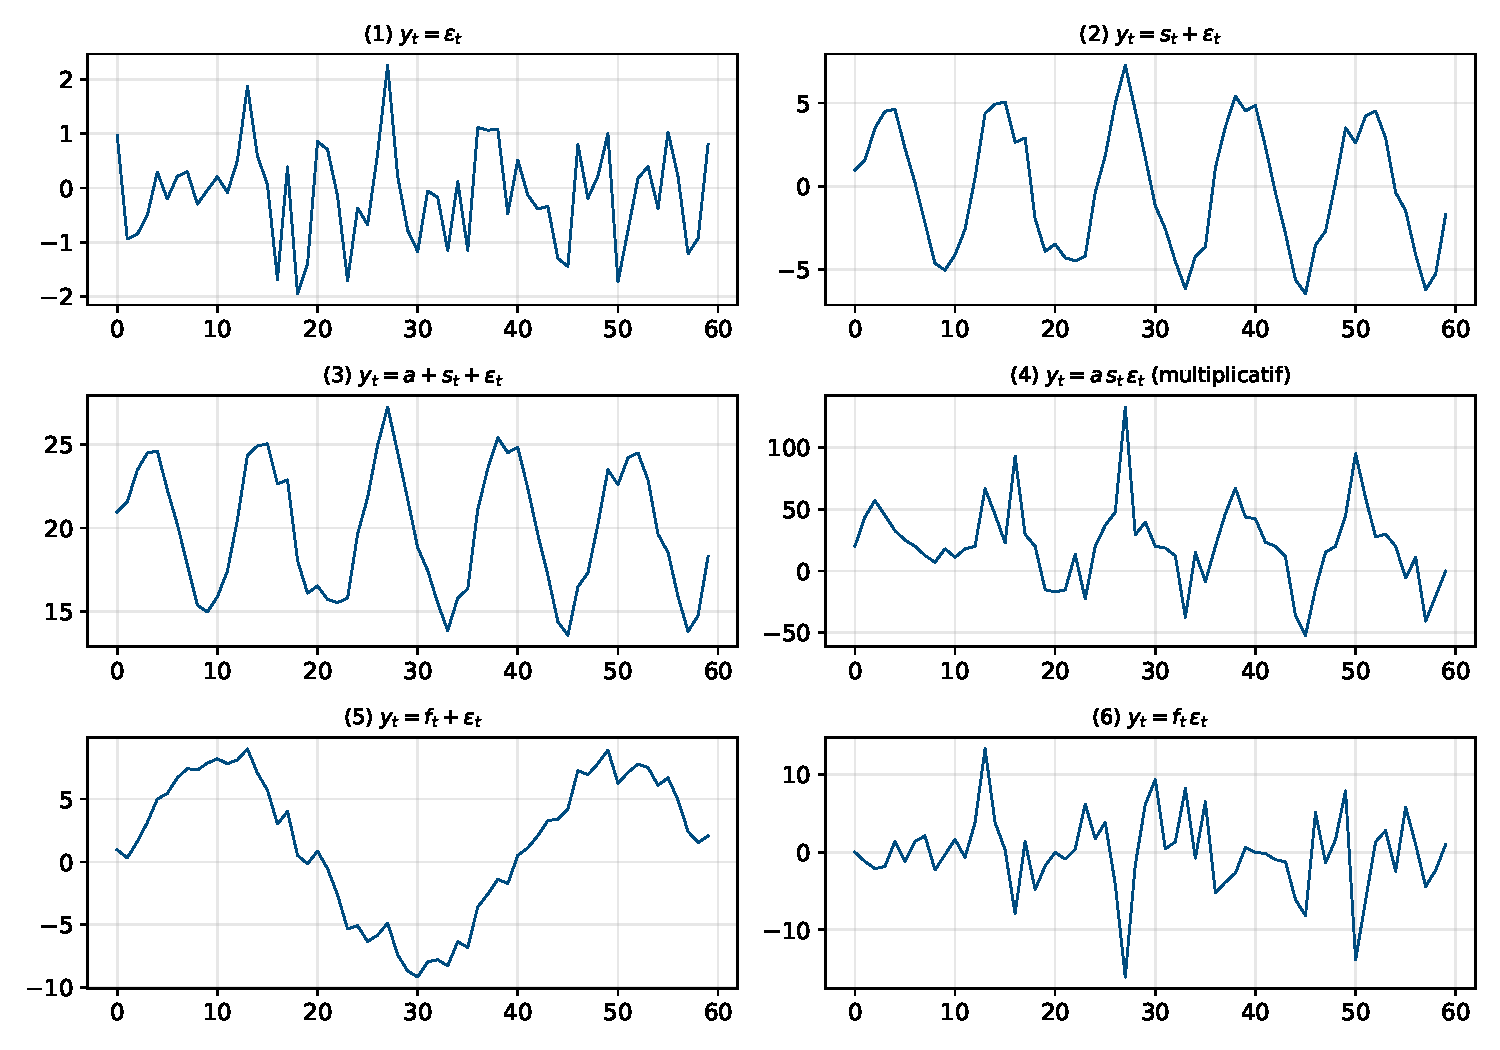
\includegraphics[width=0.95\textwidth]{identif_series.pdf}\end{center}

\item On donne les fonctions d'autocorrélation (ACF) empiriques de trois séries D, E, F.
Identifier le type de processus derrière chacune (AR, MA, ou non stationnaire), en justifiant.
\begin{center}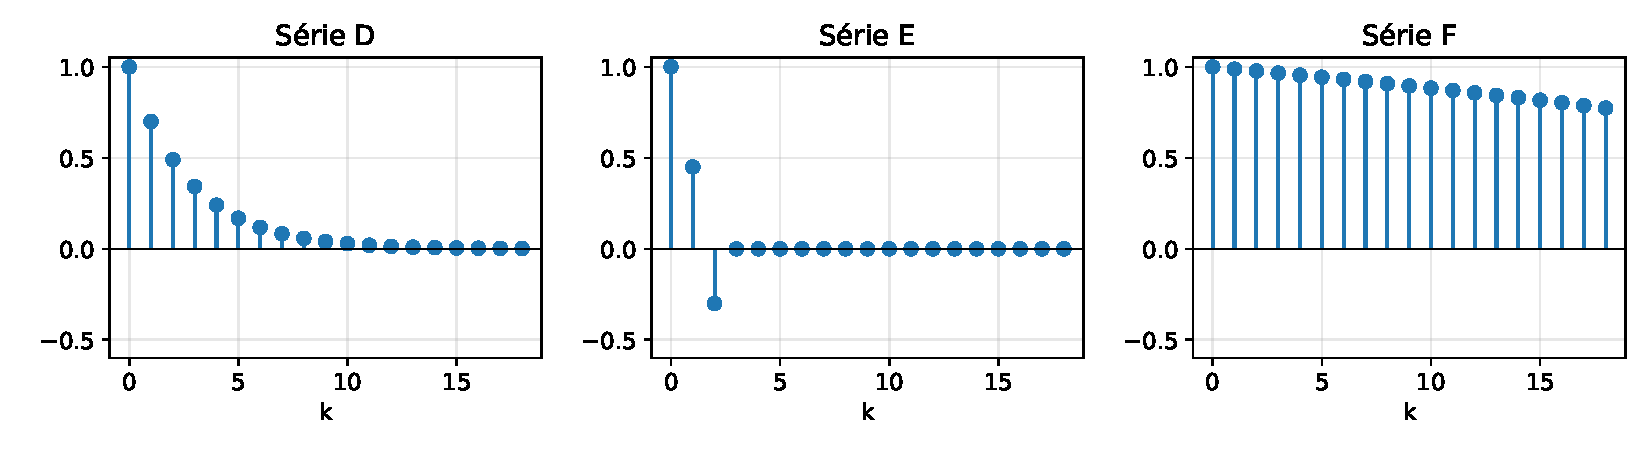
\includegraphics[width=0.97\textwidth]{identif_acf.pdf}\end{center}

\item \emph{(Examen 17/12/2019.)} Pour cinq séries dont on a tracé l'ACF et la PACF, choisir
(en justifiant) une modélisation parmi celles proposées et écrire le modèle explicite :
\emph{1)} AR(1), AR(2), MA(1), MA(2) ;
\emph{2)} AR(1), ARIMA(1,1,0), ARIMA(1,0,1), ARIMA(1,0,0) ;
\emph{3)} AR(2), AR(3), MA(2), MA(3) ;
\emph{4)} SARIMA$(2,0,1)\times(2,0,2)_{10}$, $(1,0,0)\times(2,0,2)_{10}$,
$(1,0,0)\times(1,0,3)_{10}$ ;
\emph{5)} SARIMA$(1,0,0)\times(2,0,0)_{12}$, $(0,0,0)\times(1,0,0)_{12}$,
$(1,0,0)\times(1,0,0)_{12}$.
\end{enumerate}

% =====================================================================
\section{Exercices de synthèse}
\markboth{Exercices de synthèse}{}
\begin{enumerate}[label=\textbf{Q\,J.\arabic*},leftmargin=*]
\item AR(1) $X_t=\phi X_{t-1}+\eps_t$, $\phi\ne0$, $(X_t)$ stationnaire.
\emph{1)} Laquelle n'est \emph{pas} correcte : (A) $\eps_t,X_{t-1}$ non corrélés ;
(B) $X_t,\eps_{t-1}$ non corrélés ; (C) $\eps_t,\eps_{t-1}$ non corrélés ;
(D) $X_t,\eps_t$ corrélés.
\emph{2)} Laquelle est correcte : (A) $\cor(X_t,X_{t-1})=\phi$ ; (B) $\cor(X_t,X_{t-2})=0$ ;
(C) $\cor(X_t,\eps_t)=0$ ; (D) $\cor(X_t,\eps_t)=\phi$.
\emph{3)} Pour $\sigma_\eps^2=1$, $\Var(X_t)=$ ? (A) 1 ; (B) $1-\phi^2$ ;
(C) $\frac1{1-\phi^2}$ ; (D) 0.
\emph{4)} Une seule série est stationnaire : (A) $t+X_t$ ; (B) $X_t-X_{t-1}$ ;
(C) $Y_t=X_t+Y_{t-1}$ ; (D) $Y_t=\eps_t+\phi^{-1}Y_{t-1}$.

\item AR(1) sur données journalières : on observe $-1$ hier et $+1$ aujourd'hui.
\emph{1)} Prévision pour demain ? (A) $\phi$ ; (B) $-\phi$ ; (C) 0 ; (D) $\phi+\eps$.
\emph{2)} Variance de l'erreur de prévision à deux jours ? (A) $\phi$ ; (B) 1 ;
(C) $1+\phi^2$ ; (D) $\phi^2$.

\item ARMA(1,1) $X_t=\phi X_{t-1}+\eta_t+\theta\eta_{t-1}$, $\sigma_\eta^2=\sigma^2$.
\emph{1)} CNS de stationnarité. \emph{2)} Quelle propriété est toujours vraie
(cf.\ $\rho(h)=\phi\rho(h-1)$ pour $h$ grand) ? \emph{3)} Si $\phi+\theta=0$, que devient
$(X_t)$ ?

\item AR$(p)$ stationnaire ($\phi_p\ne0$). Une seule affirmation est (en général) vraie :
(A) $\rho(h)=0$ pour $h>p$ ; (B) $P(h)=0$ pour $h>p$ ; (C) $\rho(p)\ne0$ ; (D) $\rho(p)=1$.

\item Marche aléatoire $Y_t=Y_{t-1}+\eps_t$, $\sigma_\eps^2=0.18$, $Y_t=0$ pour $t\le0$.
Écart-type de $Y_2$ ?

\item $Y_t=\tfrac12(\eps_t+\eps_{t-1})$, $\sigma_\eps^2=8$. Calculer $\Cov(Y_t,Y_{t-1})$.

\item $Y_t=\tfrac18\sum_{i=0}^{7}\eps_{t-i}$, $\sigma_\eps^2=0.64$. Calculer
$\Corr(Y_t,Y_{t-1})$.

\item AR(1) stationnaire, 200 obs., $\gammahat(0)=0.348$, $\Var(\bar Y)=0.006$. Déterminer
$\phi$. \emph{(Indication : $\Var(\bar Y)\approx\frac{\gamma(0)}{n}\frac{1+\phi}{1-\phi}$.)}

\item MA(2) $Y_t=a_t+\theta_1a_{t-1}+\theta_2a_{t-2}$, $\theta_1=0.2,\theta_2=-0.7,\sigma^2=1$.
Calculer $\Var(Y_t)$, $\Corr(Y_t,Y_{t-1})$, $\Corr(Y_t,Y_{t-2})$.

\item AR(1) $\phi=-0.5$, $\sigma_\eps=8.66$. Calculer $\Cov(Y_t,Y_{t-1})$, $\Cov(Y_t,Y_{t-2})$.

\item AR(1) $\phi>0$, $\sigma_\eps^2=5.333$, $\gamma(2)=3$. Déterminer $\phi$ et $\gamma(1)$.

\item ARMA(1,1) $X_t=\phi X_{t-1}+\eps_t+\theta\eps_{t-1}$, $\phi=-0.5,\theta=-0.6,\sigma^2=4$.
Calculer $\gamma(0),\gamma(1),\rho(1),\rho(2)$.

\item ARIMA(2,1,2)
$Y_t=1+1.8Y_{t-1}-1.4Y_{t-2}+0.6Y_{t-3}+\eps_t-0.4\eps_{t-1}+0.1\eps_{t-2}$.
Déterminer $\phi_1,\phi_2$ de la partie AR stationnaire (après différenciation).

\item $Y_t=X_t+\eps_t$ avec $X_t=X_{t-1}+u_t$ ; $(\eps_t),(u_t)$ bruits blancs indépendants,
$\sigma_\eps^2=2,\sigma_u^2=1$. Calculer $\Var(\Delta Y_t)$ et $\Corr(\Delta Y_t,\Delta Y_{t-1})$.

\item AR(2) $\phi_1=-0.5,\phi_2=-0.3$. Calculer $\rho(1),\rho(2),P(2)$.

\item AR(2), 100 obs., $\gammahat(0)=4$, $\rhohat(1)=\rhohat(2)=0.5$, $\bar Y=1$. Calculer
$\hat\sigma_\eps^2$.

\item AR(2) $\phi_1=0.5,\phi_2=0.3$, moyenne $\mu=5$ ; $Y_1=5,Y_2=7,Y_3=5$. Calculer la
meilleure prévision $\widehat Y_4$.

\item $Y_t=X_t+V_t$, $X_t$ AR(1) $X_t=\phi X_{t-1}+a_t$, $V_t,a_t$ bruits blancs indépendants
de variances $\sigma_v^2,\sigma_a^2$. \emph{1)} Autocovariance de $Y_t$. \emph{2)}
Stationnaire ?

\item \emph{(Rattrapage 2024--2025.)} $y_t=x_t+v_t$, $x_t=\phi x_{t-1}+u_t$, $|\phi|<1$,
$v_t,u_t$ bruits blancs indépendants ; $\phi=0.5,\sigma_v^2=0.25,\sigma_u^2=1$.
\emph{a)} Autocovariance de $y_t$ ; stationnaire ? \emph{b)} $z_t=y_t-\phi y_{t-1}$ :
calculer $\gamma_z(k)$ et identifier le(s) ARMA$(p,q)$. \emph{c)} Donner $\theta$ et
$\sigma_e^2$ (quelle solution retenir ?).

\item \emph{(Rattrapage 2024--2025.)} $x_t=a_t-\theta a_{t-2}$, $\sigma_a^2=1$, $\theta=0.8$,
$m=\tfrac14(x_1+x_2+x_3+x_4)$. Calculer $\Var(m)$.

\item Après estimation d'un ARMA(1,1) sur 100 points, la statistique de Ljung--Box sur les 14
premières autocorrélations des résidus vaut $\mathrm{LB}=18.386$. Conclusion ? (rejet / non
rejet de $H_0$). Justifier.
\end{enumerate}

% =====================================================================
\section{Hors programme du cours BADAOUI\,\texorpdfstring{\horsprog}{*}}
\markboth{Hors programme}{}
\begin{tcolorbox}[colback=orangelight,colframe=orange,title={Avertissement}]
Notions \emph{non couvertes} par le cours BADAOUI (issues d'autres sources : QCM Charpentier,
examens INSEA 2016/2017 et 17/12/2019, OpenClassroom). Traitées à part dans le corrigé.
\end{tcolorbox}
\begin{enumerate}[label=\textbf{Q\,Z.\arabic*},leftmargin=*]
\item \textbf{Bruit blanc fort/faible.} $(\eta_t)$ i.i.d.\ centrée de variance 1 ;
$\eps_t=\eta_t\eta_{t-1}\eta_{t-2}$. Montrer que $(\eps_t)$ est un bruit blanc, dire s'il est
fort ou faible, et montrer que $(\eps_t^2)$ suit un ARMA.
\item \textbf{Stationnarité mutuelle.} Conditions pour que deux processus $X,Y$ soient
mutuellement (conjointement) stationnaires (cocher).
\item \textbf{Inverses d'opérateurs.} Donner $(I-\tfrac15 B)^{-1}$ et $(I+3B)^{-1}$ (préciser
le domaine de validité).
\item \textbf{Projection orthogonale (17/12/2019).} $\Phi(B)=I-\tfrac16B-\tfrac16B^2$.
\emph{1)} Inversibilité et inverse. \emph{2)} $\Phi(B)X_t=\eps_t$ : type, stationnarité,
$\mathrm{MA}(\infty)$, $\gamma$, loi de $(X_t,X_{t+3})$ (cas gaussien). \emph{3)}
$\Phi(B)Y_t=\eps_t-\tfrac13\eps_{t-1}$ : type, minimalité, innovations, $\mathrm{AR}(\infty)$,
projection sur le passé.
\item \textbf{Lissage / filtres (QCM).} \emph{1)} Le lissage exponentiel simple ajuste
localement une constante (V/F). \emph{2)} Holt--Winters intègre la saisonnalité (V/F).
\emph{3)} Pour estimer une tendance $m$ en présence de saisonnalité $s$, le filtre doit
absorber $s$ et laisser $m$ (quelle option ?). \emph{4)} Pour tester la blancheur des résidus
(AIC / ACF-PACF / Ljung--Box / moyenne mobile ?).
\end{enumerate}

\end{document}
